\documentclass[a4paper]{report}
% Some basic packages
\usepackage[utf8]{inputenc}
\usepackage[T1]{fontenc}
\usepackage{textcomp}
\usepackage[english]{babel}
\usepackage{url}
\usepackage{graphicx}
\usepackage{float}
\usepackage{booktabs}
\usepackage{enumitem}

\pdfminorversion=7

% Don't indent paragraphs, leave some space between them
\usepackage{parskip}

% Hide page number when page is empty
\usepackage{emptypage}
\usepackage{subcaption}
\usepackage{multicol}
\usepackage{xcolor}

% Other font I sometimes use.
% \usepackage{cmbright}

% Math stuff
\usepackage{amsmath, amsfonts, mathtools, amsthm, amssymb}
% Fancy script capitals
\usepackage{mathrsfs}
\usepackage{cancel}
% Bold math
\usepackage{bm}
% Some shortcuts
\newcommand\N{\ensuremath{\mathbb{N}}}
\newcommand\R{\ensuremath{\mathbb{R}}}
\newcommand\Z{\ensuremath{\mathbb{Z}}}
\renewcommand\O{\ensuremath{\emptyset}}
\newcommand\Q{\ensuremath{\mathbb{Q}}}
\newcommand\C{\ensuremath{\mathbb{C}}}
\renewcommand\L{\ensuremath{\mathcal{L}}}

% Package for Petri Net drawing
\usepackage[version=0.96]{pgf}
\usepackage{tikz}
\usetikzlibrary{arrows,shapes,automata,petri}
\usepackage{tikzit}
\input{petri_nets_style.tikzstyles}

% Easily typeset systems of equations (French package)
\usepackage{systeme}

% Put x \to \infty below \lim
\let\svlim\lim\def\lim{\svlim\limits}

%Make implies and impliedby shorter
\let\implies\Rightarrow
\let\impliedby\Leftarrow
\let\iff\Leftrightarrow
\let\epsilon\varepsilon

% Add \contra symbol to denote contradiction
\usepackage{stmaryrd} % for \lightning
\newcommand\contra{\scalebox{1.5}{$\lightning$}}

% \let\phi\varphi

% Command for short corrections
% Usage: 1+1=\correct{3}{2}

\definecolor{correct}{HTML}{009900}
\newcommand\correct[2]{\ensuremath{\:}{\color{red}{#1}}\ensuremath{\to }{\color{correct}{#2}}\ensuremath{\:}}
\newcommand\green[1]{{\color{correct}{#1}}}

% horizontal rule
\newcommand\hr{
    \noindent\rule[0.5ex]{\linewidth}{0.5pt}
}

% hide parts
\newcommand\hide[1]{}

% si unitx
\usepackage{siunitx}
\sisetup{locale = FR}

% Environments
\makeatother
% For box around Definition, Theorem, \ldots
\usepackage{mdframed}
\mdfsetup{skipabove=1em,skipbelow=0em}
\theoremstyle{definition}
\newmdtheoremenv[nobreak=true]{definitie}{Definitie}
\newmdtheoremenv[nobreak=true]{eigenschap}{Eigenschap}
\newmdtheoremenv[nobreak=true]{gevolg}{Gevolg}
\newmdtheoremenv[nobreak=true]{lemma}{Lemma}
\newmdtheoremenv[nobreak=true]{propositie}{Propositie}
\newmdtheoremenv[nobreak=true]{stelling}{Stelling}
\newmdtheoremenv[nobreak=true]{wet}{Wet}
\newmdtheoremenv[nobreak=true]{postulaat}{Postulaat}
\newmdtheoremenv{conclusie}{Conclusie}
\newmdtheoremenv{toemaatje}{Toemaatje}
\newmdtheoremenv{vermoeden}{Vermoeden}
\newtheorem*{herhaling}{Herhaling}
\newtheorem*{intermezzo}{Intermezzo}
\newtheorem*{notatie}{Notatie}
\newtheorem*{observatie}{Observatie}
\newtheorem*{exe}{Exercise}
\newtheorem*{opmerking}{Opmerking}
\newtheorem*{praktisch}{Praktisch}
\newtheorem*{probleem}{Probleem}
\newtheorem*{terminologie}{Terminologie}
\newtheorem*{toepassing}{Toepassing}
\newtheorem*{uovt}{UOVT}
\newtheorem*{vb}{Voorbeeld}
\newtheorem*{vraag}{Vraag}

\newmdtheoremenv[nobreak=true]{definition}{Definition}
\newtheorem*{eg}{Example}
\newtheorem*{notation}{Notation}
\newtheorem*{previouslyseen}{As previously seen}
\newtheorem*{remark}{Remark}
\newtheorem*{note}{Note}
\newtheorem*{problem}{Problem}
\newtheorem*{observe}{Observe}
\newtheorem*{property}{Property}
\newtheorem*{intuition}{Intuition}
\newmdtheoremenv[nobreak=true]{prop}{Proposition}
\newmdtheoremenv[nobreak=true]{theorem}{Theorem}
\newmdtheoremenv[nobreak=true]{corollary}{Corollary}

% End example and intermezzo environments with a small diamond (just like proof
% environments end with a small square)
\usepackage{etoolbox}
\AtEndEnvironment{vb}{\null\hfill$\diamond$}%
\AtEndEnvironment{intermezzo}{\null\hfill$\diamond$}%
% \AtEndEnvironment{opmerking}{\null\hfill$\diamond$}%

% Fix some spacing
% http://tex.stackexchange.com/questions/22119/how-can-i-change-the-spacing-before-theorems-with-amsthm
\makeatletter
\def\thm@space@setup{%
  \thm@preskip=\parskip \thm@postskip=0pt
}


% Exercise 
% Usage:
% \exercise{5}
% \subexercise{1}
% \subexercise{2}
% \subexercise{3}
% gives
% Exercise 5
%   Exercise 5.1
%   Exercise 5.2
%   Exercise 5.3
\newcommand{\exercise}[1]{%
    \def\@exercise{#1}%
    \subsection*{Exercise #1}
}

\newcommand{\subexercise}[1]{%
    \subsubsection*{Exercise \@exercise.#1}
}


% \lecture starts a new lecture (les in dutch)
%
% Usage:
% \lecture{1}{di 12 feb 2019 16:00}{Inleiding}
%
% This adds a section heading with the number / title of the lecture and a
% margin paragraph with the date.

% I use \dateparts here to hide the year (2019). This way, I can easily parse
% the date of each lecture unambiguously while still having a human-friendly
% short format printed to the pdf.

\usepackage{xifthen}
\def\testdateparts#1{\dateparts#1\relax}
\def\dateparts#1 #2 #3 #4 #5\relax{
    \marginpar{\small\textsf{\mbox{#1 #2 #3 #5}}}
}

\def\@lecture{}%
\newcommand{\lecture}[3]{
    \ifthenelse{\isempty{#3}}{%
        \def\@lecture{Lecture #1}%
    }{%
        \def\@lecture{Lecture #1: #3}%
    }%
    \subsection*{\@lecture}
    \marginpar{\small\textsf{\mbox{#2}}}
}



% These are the fancy headers
\usepackage{fancyhdr}
\pagestyle{fancy}

% LE: left even
% RO: right odd
% CE, CO: center even, center odd
% My name for when I print my lecture notes to use for an open book exam.
% \fancyhead[LE,RO]{Gilles Castel}

\fancyhead[RO,LE]{\@lecture} % Right odd,  Left even
\fancyhead[RE,LO]{}          % Right even, Left odd

\fancyfoot[RO,LE]{\thepage}  % Right odd,  Left even
\fancyfoot[RE,LO]{}          % Right even, Left odd
\fancyfoot[C]{\leftmark}     % Center

\makeatother




% Todonotes and inline notes in fancy boxes
\usepackage{todonotes}
\usepackage{tcolorbox}

% Make boxes breakable
\tcbuselibrary{breakable}

% Verbetering is correction in Dutch
% Usage: 
% \begin{verbetering}
%     Lorem ipsum dolor sit amet, consetetur sadipscing elitr, sed diam nonumy eirmod
%     tempor invidunt ut labore et dolore magna aliquyam erat, sed diam voluptua. At
%     vero eos et accusam et justo duo dolores et ea rebum. Stet clita kasd gubergren,
%     no sea takimata sanctus est Lorem ipsum dolor sit amet.
% \end{verbetering}
\newenvironment{verbetering}{\begin{tcolorbox}[
    arc=0mm,
    colback=white,
    colframe=green!60!black,
    title=Opmerking,
    fonttitle=\sffamily,
    breakable
]}{\end{tcolorbox}}

% Noot is note in Dutch. Same as 'verbetering' but color of box is different
\newenvironment{noot}[1]{\begin{tcolorbox}[
    arc=0mm,
    colback=white,
    colframe=white!60!black,
    title=#1,
    fonttitle=\sffamily,
    breakable
]}{\end{tcolorbox}}




% Figure support as explained in my blog post.
\usepackage{import}
\usepackage{xifthen}
\usepackage{pdfpages}
\usepackage{transparent}
\newcommand{\incfig}[1]{%
    \def\svgwidth{\columnwidth}
    \import{./figures/}{#1.pdf_tex}
}

% Fix some stuff
% %http://tex.stackexchange.com/questions/76273/multiple-pdfs-with-page-group-included-in-a-single-page-warning
\pdfsuppresswarningpagegroup=1


% My name
\author{Bruno M. Pacheco}

\newenvironment{alltt}{\ttfamily}{\par}
 
\begin{document}
 
\title{Production Optimization of Gas-Lifted Oil Wells}
\author{Bruno M. Pacheco (202100361) \\
DAS410062 - Introduction to Optimization}
 
\maketitle
 
\section{Introduction}

This report details the MILP formulation and implementation of the proposed gas-lift rate optimization problem as well as the results found. This problem's main challenge regards its non-linear nature from the relationship between the injected gas and the produced oil. Therefore, piecewise linearization techniques were applied so we can bring the problem into the linear domain, achieving approximated results. Beside the discontinuities that the linearization methods bring, the option to produce or not from any given well introduces binary variables which result in the mixed-integer formulation.

The implementation of the proposed formulations was completely done in AMPL and the solver used for the optimization was CPLEX (running on local machine). All of the developed code and raw results are made available with this document.

\section{Reformulations}

\subsection{Convex Combination}

By applying the Convex Combination method to the $q_o^{n}\left( q_{inj}^n \right) $ relations of each well one achieves a reformulation that replaces (2f) (as in the assignment description) by
\begin{align*}
    &q_{inj}^{n} = \sum_{i=1}^{K^{n}} \lambda^{n,i} q_{inj}^{n,i} \\
    &\dot{q}_o^{n} = \sum_{i=1}^{K^{n}} \lambda^{n,i} q_o^{n,i} \\
    &1 = \sum_{i=1}^{K^{n}} \lambda^{n,i} \tag{$*$}\\
    &1 = \sum_{i=2}^{K^{n}} z^{n,i} \\
    &\lambda^{n,i} \le z^{n,i} + z^{n,i+1},\, i=2,\ldots,K^{n}-1 \\
    &\lambda^{n,1} \le z^{n,2},\, \lambda^{n,K^{n}} \le z^{n,K^{n}}
,\end{align*}
for each $n \in \mathcal{N}$, where $\lambda^{n,i}$ are non-negative and $z^{n,i}$ are binary variables and $\mathcal{K}^{n} = \left\{  \left( q_{inj}^{n,1}, q_o^{n,1} \right), \ldots, \left( q_{inj}^{n,K^{n}}, q_o^{n,K^{n}} \right) \right\} $ are the data points for each $q_o^{n}\left( q_{inj}^n \right)$ function.

Now, note that the use of the $y^{n}$ variables to control which wells are in use together with equation (2g) result in $y^{n} = 0 \implies q_{inj}^{n} = 0$, and the desired behavior would be for $y^{n}=0 \implies \dot{q}_o^{n} = 0$. Still, the CC constraints enforce that $\dot{q}_o^{n} \ge \min \left\{ q_o^{n,1},\ldots,q_o^{n,K^{n}} \right\} $, which, in case of surgent wells, is a positive value. Therefore, to avoid such scenarios, the constraint \[
\hat{q}_o^{n} = \dot{q}_o^{n} - \left( 1 - y^{n} \right) q_o^{n,1},\, n\in \mathcal{N}
\] 
is added.

\subsection{SOS2}

If we have access to Special Ordered Sets of type 2 (SOS2) as a type for the variables in our solver, then our piecewise linearization can become much lighter. In practice, the constraints in $\left( * \right) $ can be replaced by
\begin{align*}
    &q_{inj}^{n} = \sum_{i=1}^{K^{n}} \lambda^{n,i} q_{inj}^{n,i} \\
    &\dot{q}_o^{n} = \sum_{i=1}^{K^{n}} \lambda^{n,i} q_o^{n,i} \\
    &1 = \sum_{i=1}^{K^{n}} \lambda^{n,i}
\end{align*}
in the MILP formulation just by adding the guarantee that each set $\left\{ \lambda^{n,i} \right\}_{i=1}^{K^{n}} $ is SOS2.

Effectively, using SOS2 variables showed a reduction in the number of variables (after presolve) from 148 to 102, on the average scenarios ($q_{inj}^{max} \ge 200$), and around 30\% less simples iterations to find the optimal solution.

\section{Results}

The behavior of the problem instance proposed is first studied through the analysis of the relation between lift-gas capacity and the total oil production. Then, 3 scenarios are analysed in depth.

Given the AMPL implementation of the problem, 30 executions of the solver were performed with lift-gas capacities ranging from 50 to 1500 in steps of 50. The impact of such in the oil production can be seen in the graph below.

\begin{figure}[H]
    \centering
    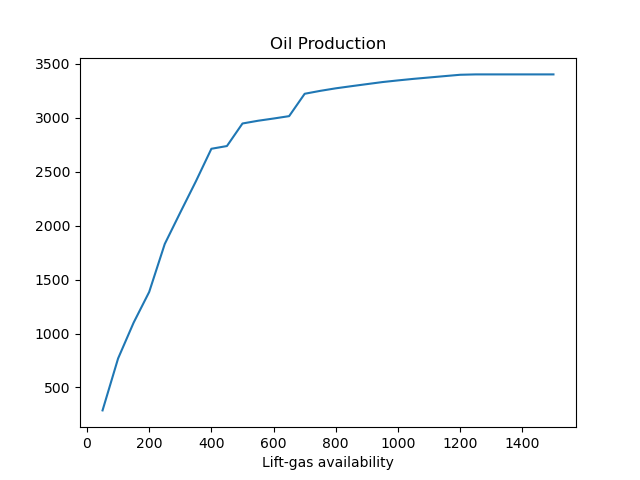
\includegraphics[width=0.8\textwidth]{oil_production.png}
    \caption{Maximum oil production as a function of lift-gas availability.}
    \label{fig:oil_production-png}
\end{figure}

As one can see, the oil production increases rapidly with the availability of lift-gas but achieves a plateau at around 1200. From this graph, first the scenario with very little lift gas is analysed in depth. For $q_{inj}^{max} = 50$, the maximum oil production is only of 286.7 and only well 5 is in production. This is caused by $q_{inj}^{min,n}$, which restrict the pool of wells to only wells 4 and 5. From these, well 5 has a higher return rate and, thus, it is the destination of all of the lift-gas. In this scenario, well 5 operates with $q_w^{5} = 4.6$ and $q_g^{5} = 1059.3$, which are still far from the respective limits of the production plant.

With $q_{inj}^{max} = 500$, there is enough lift-gas to put all but the well 1 in operation, resulting in a total oil production of 2948.1. Still, the lift-gas availability is the bottle-neck as the bare minimum of gas-lift is used in all wells in production but for wells 3 and 8 (analysis of the slack of the constraint). The operating conditions for each well in production can be seen in the table below.

\begin{table}[H]
    \centering
    \begin{tabular}{c|c|c|c|c}
	Well & $q_{inj}^{n}$ & $q_o^{n}$ & $q_w^{n}$ & $q_g^{n}$ \\
	\hline
	2 & 68 & 530 & 493.957 & 380.964 \\
	3 & 70 & 486.072 & 410.575 & 294.171 \\
	4 & 42 & 284 & 167.941 & 852 \\
	5 & 35 & 285 & 4.60471 & 1053.13 \\
	6 & 74 & 315 & 167.685 & 434.637 \\
	7 & 114 & 815 & 83.9632 & 536.84 \\
	8 & 97 & 233 & 37.3016 & 510.713
    \end{tabular}
    \caption*{Operating conditions of the wells in production for $q_{inj}^{max} = 500$.}
    \label{tab:label}
\end{table}

Finally, for $q_{inj}^{max} = 1500$, there is a total oil production of 3403.4 and all the wells are in production. In this scenario with plenty lift-gas, the bottle-neck of production becomes $q_g^{max}$, which makes so that no one of the wells produce in its full capacity and wells 4 to 7 still operate with the bare minimum lift-gas consumption. The operating conditions of the wells are in the table below.

\begin{table}[H]
    \centering
    \begin{tabular}{c|c|c|c|c}
	Well & $q_{inj}^{n}$ & $q_o^{n}$ & $q_w^{n}$ & $q_g^{n}$ \\
	\hline
	1 & 314 & 324 & 272.356 & 636.401 \\
	2 & 266 & 591 & 550.808 & 424.811 \\
	3 & 272.703 & 556.449 & 470.02 & 336.763 \\
	4 & 42 & 284 & 167.941 & 852 \\
	5 & 35 & 285 & 4.60471 & 1053.13 \\
	6 & 74 & 315 & 167.685 & 434.637 \\
	7 & 114 & 815 & 83.9632 & 536.84 \\
	8 & 97 & 233 & 37.3016 & 510.713 \\
    \end{tabular}
    \caption*{Operating conditions of the wells in production for $q_{inj}^{max} = 1500$.}
    \label{tab:label}
\end{table}


\end{document}
